\chapter{Harmonogram Realizacji Projektu}

Harmonogram realizacji projektu został zaplanowany z wykorzystaniem diagramu Gantta, który ilustruje kluczowe etapy rozwoju projektu, ich zależności czasowe oraz alokację zasobów. Poniżej przedstawiono diagram Gantta dla projektu aplikacji pozwalającej na szybkie sprawdzenie wersji serwisów na serwerach Linux.

\begin{figure}[H]
\centering
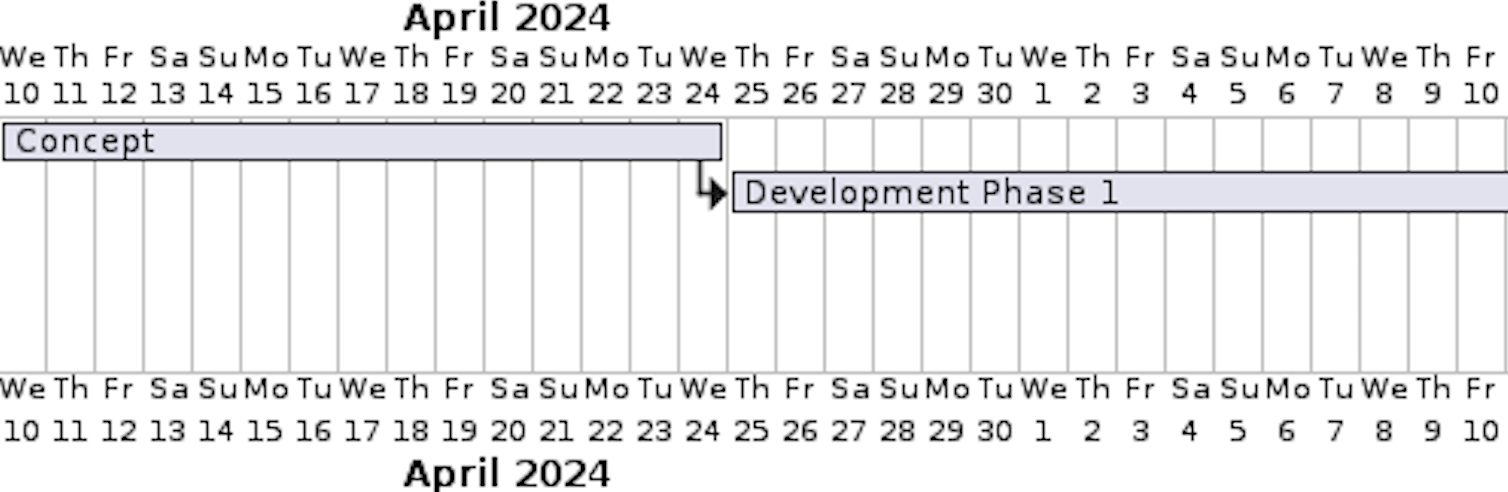
\includegraphics[width=\textwidth]{photos/Gant1.png}
\caption{Diagram Gantta}
\end{figure}
\begin{figure}[H]
\centering
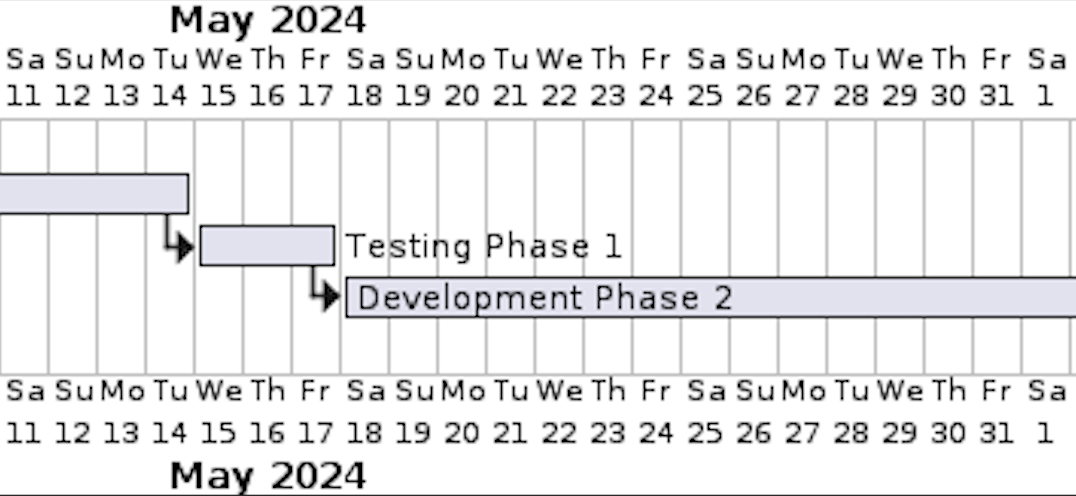
\includegraphics[width=\textwidth]{photos/Gant2.png}
\caption{Diagram Gantta}
\end{figure}
\begin{figure}[H]
\centering
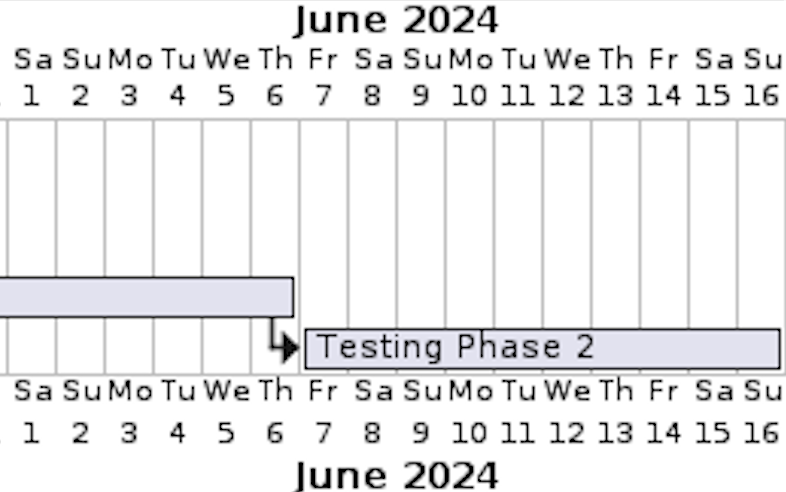
\includegraphics[width=0.80\textwidth]{photos/Gant3.png}
\caption{Diagram Gantta}
\end{figure}
